\section{Conclusion}
\label{sec:conclusion}

In this laboratory assignment the objective of building an AC/DC converter circuit by using a tranformer, envelope detetcor and a low-pass filter was achieved.
 The ripple has a value of $4.13*10^{-3} V$.
 The stabilization time was of around 1 second.
 The cost of the circuit was of $59.9448 MU$.
 The merit is therefore equal to $4.03825$
 
The results from both the theoretical analysis using octave and the circuit
simulation using ngspice appear to match as can be seen in the below comparison:

\begin{minipage}[c]{0.50\linewidth}
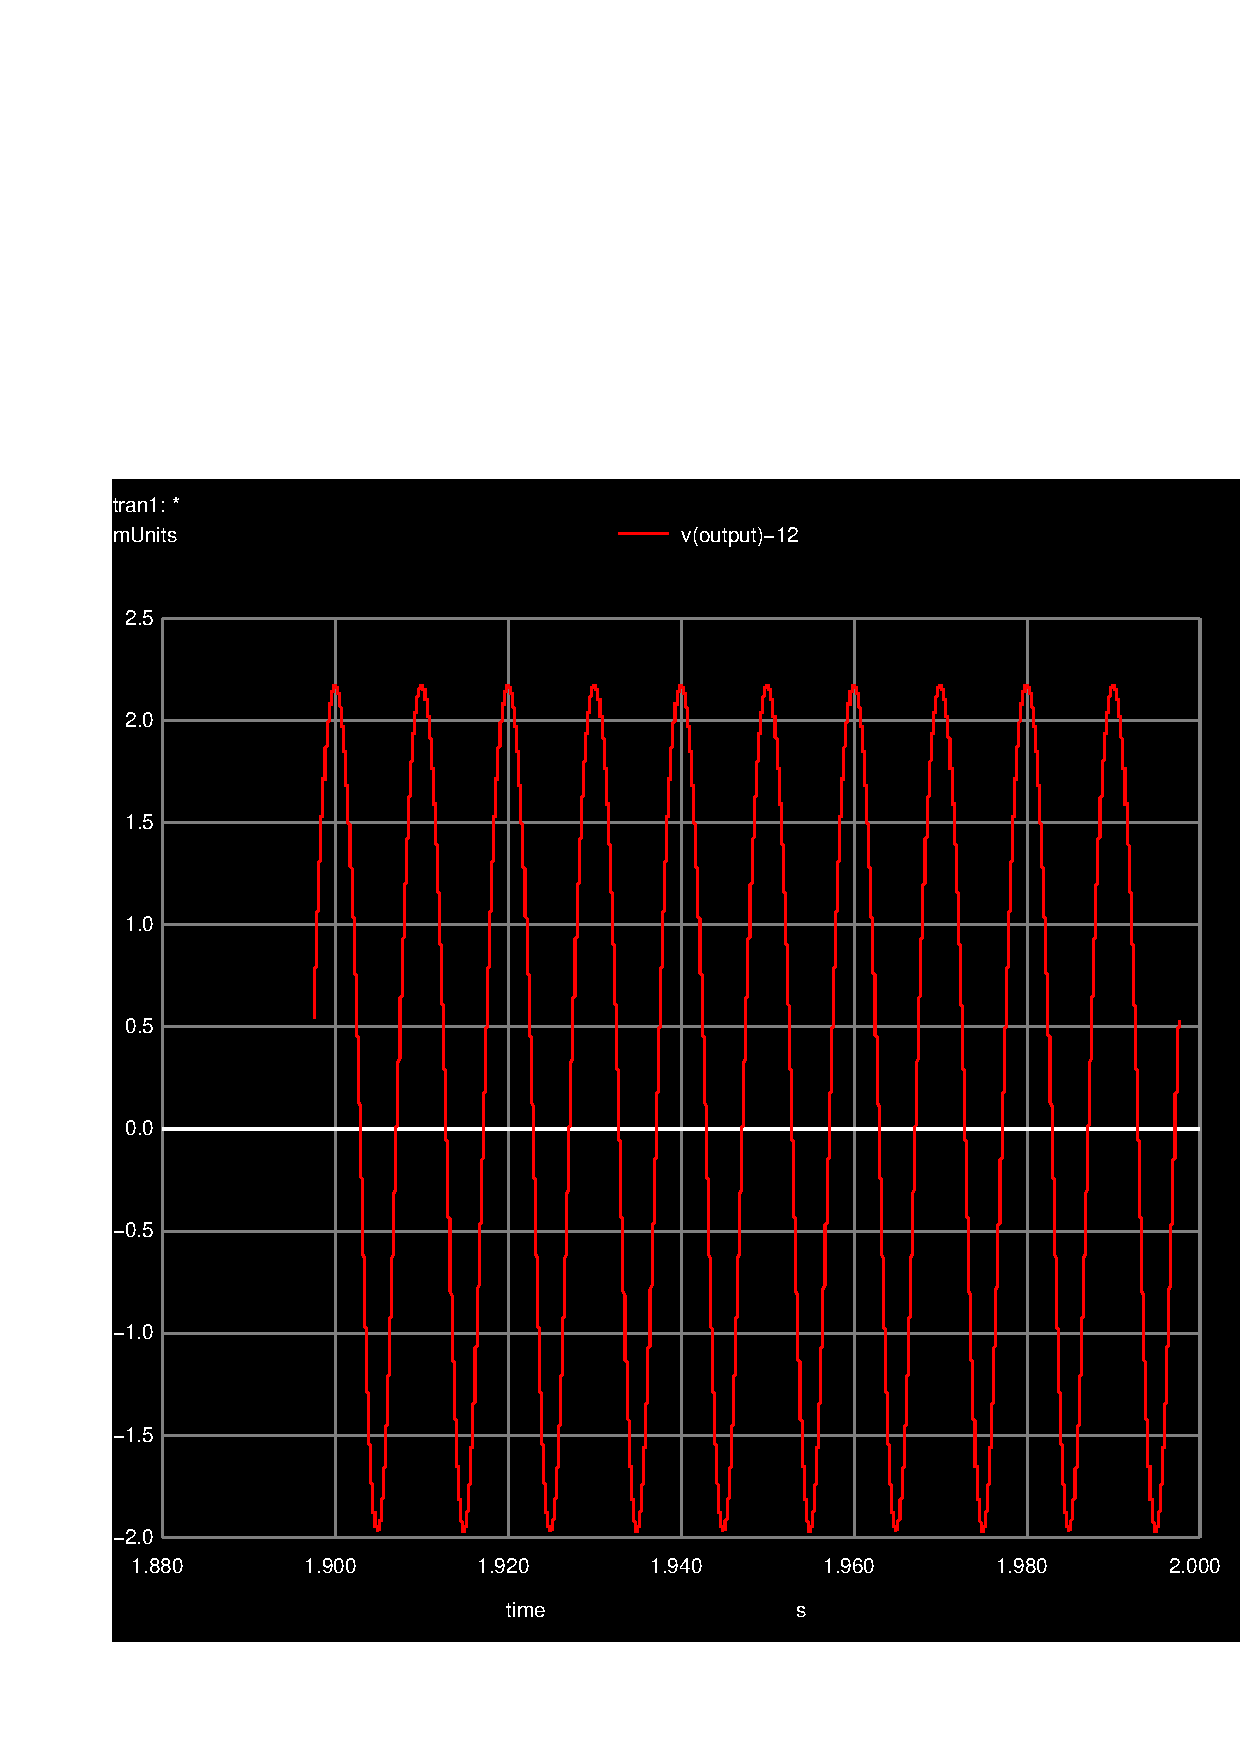
\includegraphics[width=1\linewidth]{../sim/v12.pdf}
\end{minipage} % no space if you would like to put them side by side
\hspace{1mm}
\begin{minipage}[c]{0.50\linewidth}
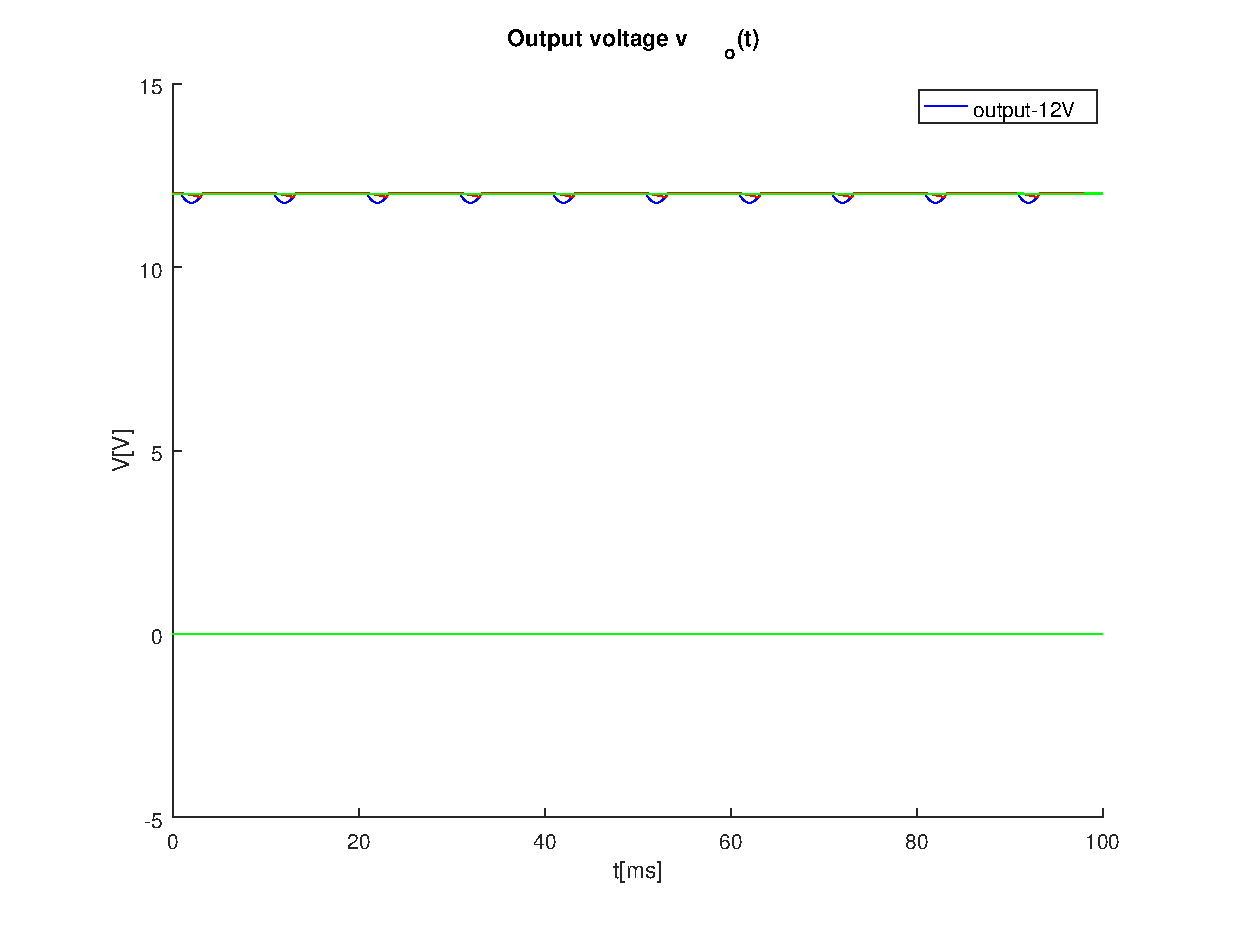
\includegraphics[width=1\linewidth]{v12.eps}
\end{minipage}
